%\documentclass[12pt]{report}
%\documentclass[12pt]{extreport}
\documentclass[17pt]{article}
\usepackage{graphicx}
\usepackage{setspace}
\usepackage{amsmath,amssymb}
\usepackage{IEEEtrantools}
\usepackage{cancel}
\usepackage[font=small,labelfont=bf]{caption}

\usepackage{sectsty}

\sectionfont{\fontsize{12}{15}\selectfont}

\usepackage{geometry}
 \geometry{
 a4paper,
 total={170mm,264mm},
 left=20mm,
 top=10mm,
 }

\begin{document}

\begin{center}
	{\bf Formulario di elettromagnetismo (aggiornato al 14/05/2020})
\end{center}


\section{Forza elettrostatica}


\begin{itemize}
	\item Legge di Coulomb         
		\begin{itemize}
			\item $F = k\cdot\frac{qQ}{r^2}$\\
			La forza di interazione \'e proporzionale al prodotto delle cariche e inversamente proporzionale al \emph{quadrato} della distanza.
		\end{itemize}			
	\item $k = 9\cdot 10^{9}$ Costante di proporzionalit\'a        
\end{itemize}



\begin{figure}[th]
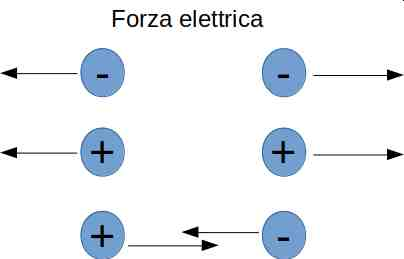
\includegraphics[width=6cm]{forzaElettrica.jpg}
\centering
\end{figure}






\subsection{Campo elettrico}

Separo l'equazione della Legge di Coulomb in due differenti equazioni:
      
\begin{itemize}
	\item $E = k\cdot\frac{Q}{r^2}$ 
	\item $F = qE$
\end{itemize}			


\begin{figure}[th]
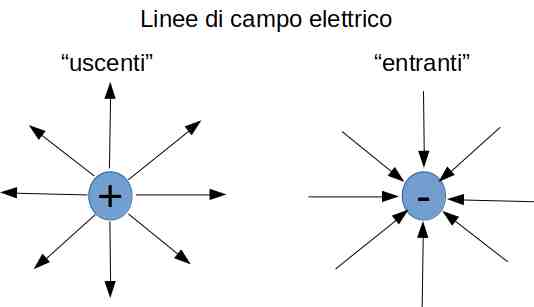
\includegraphics[width=8cm]{lineeCampoElettrico.jpg}
\centering
\end{figure}






\section{Forza magnetica}

\begin{itemize}
	\item Forza magnetica tra due fili percorsi da corrente elettrica $i$ e $I$ rispettivamente: $F = k_m \frac{iI}{d}$\\
	La forza di interazione tra due fili percorsi da corrente elettrica \'e proporzionale al prodotto delle correnti elettriche e inversamente proporzionale alla distanza. Il coefficiente di proporzionalit\'a \'e $k_m$.
	\begin{itemize}
		\item $k_m = 796000$ costande di proporzionalit\'a
		\item l = lunghezza dei due fili
		\item d = distanza tra i due fili
	\end{itemize}
\end{itemize}


\begin{figure}[th]
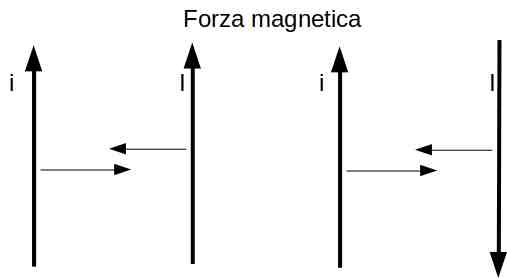
\includegraphics[width=8cm]{forzaMagnetica.jpg}
\centering
\end{figure}


\subsection{Campo magnetico}
Il campo magnetico \'e un \emph{campo vettoriale} $\vec{B}$

\begin{itemize}
	\item $B = k_m \frac{I}{d}$ campo magnetico generato da un filo percorso da corrente $I$.
	\item $F = iBl$ Forza su un filo percorso da corrente $i$, dovuto alla presenza di un campo magnetico $B$ \emph{perpendicolare}.
\end{itemize}





\section{Resistenze elettriche}

\begin{itemize}
	\item Prima Legge di Ohm $V = Ri$
		\begin{itemize}
			\item V = Tensione, si esprime in Volt (V)
			\item R = Resistenza elettrica, si esprime in Ohm ($\Omega$)
			\item i = Intensit\'a di corrente elettrica, si esprime in Ampere (A)
		\end{itemize}
	\item Seconda Legge di Ohm $R=\rho\frac{l}{A}$
		\begin{itemize}
			\item R = Resistenza elettrica
			\item $\rho$ = Resistivit\'a, diversa per ogni materiale
			\item l = lunghezza
			\item A = Sezione
		\end{itemize}
	\item Serie $R_{eq} = R_1 + R_2$
	\item Parallelo $\frac{1}{R_{eq}} = \frac{1}{R_1} + \frac{1}{R_2}$
	\item Prima Legge di Kirchhoff: in un \emph{nodo} la somma delle correnti entranti \'e uguale alla somma delle correnti uscenti
	\item Seconda Legge di Kirchhoff: in una \emph{maglia} la somma delle cadute di potenziale \'e nulla
\end{itemize}





\section{Onde elettromagnetiche}

Il dipolo elettrico \'e costituito da due cariche di uguale intensit\'a ma opposte tra loro e disposte molto vicine l'una rispetto all'altra. Il dipolo \'e un sistema elettricamente carico ma che genera un campo elettrico \emph{non nullo} intorno a se. La molecola dell'acqua \'e un esempio di dipolo elettrico. Quando un dipolo elettrico oscilla, genera intorno a se una \emph{perturbazione del campo elettromagnetico che si propaga nello spazio e nel tempo} ad una velocit\'a $c = 3\cdot 10^{8}m/s$. Tale perturbazione si chiama \emph{onda elettromagnetica}.

\begin{figure}[th]
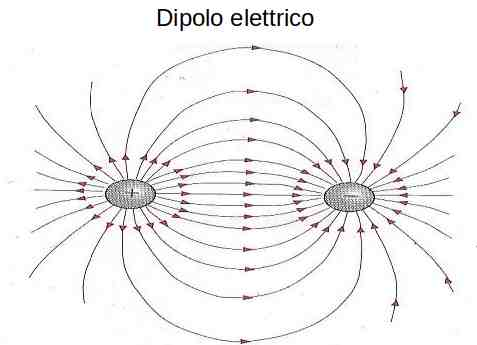
\includegraphics[width=8cm]{dipoloElettrico.jpg}
\centering
\end{figure}

\end{document}